\documentclass[a4paper]{article}
\usepackage{gensips,amsmath,epsfig}
\usepackage{graphicx}

% Example definitions.
% --------------------
\def\x{{\mathbf x}}
\def\L{{\cal L}}

% Title.
% ------
\title{CSCI 5471 - Report\\
IMPLEMENTING SIA PROTOCOL IN TINYDB/TINYOS AND \\
SURVEY ON PROTOCOLS FOR SECURE DATA AGGREGATION IN WSN}

%
% Single address.
% ---------------
%\name{Author(s) Name(s)\thanks{Thanks to XYZ agency for funding.}}
%\address{Author Affiliation(s)}
%
% For example:
% ------------
%\address{Department, School\\
%   Address\\
%   email addresses}
%
% If there are multiple departments then they should be marked as below.
\name{Brian Kleinke, Matt Kokotovich, Thanh Ngo, Matt Soukup and  Yul-Duck Sung}
\address{Department of Computer Science and Engineering\\
University of Minnesota, Twin Cities \\
\{klein399,kokot012,ngotr001,souku024,sungx069\}@umn.edu }
\hyphenation{col-umns}

\begin{document}

%
\maketitle

%
%\begin{abstract}

%Need for an abstract?

%\end{abstract}

%
\section{Introduction}
\label{sec:intro}

In today's world, wireless sensor networks (WSN) are becoming increasingly
common with the rapid improvement in wireless data transmission networks and
the miniaturization of components. They were originally developed and used by
the military; today, they are used in many civilian and industry applications,
as well. Due to technological advances characterized by Moore's law, we now
have small, incredibly powerful monitoring devices, which use a wireless
network to transmit data. We are motivated by both this advance in technology
an increase in the power of network monitor tools to improve on existing WSN
secure data aggregation protocols. We believe that this field still contains
areas for improvement. We became interested in combining protocols after
reading Wireless Sensor Network Security: A Survey[8] and Secure Data
Aggregation in Wireless Sensor[9] from which one can gain a good overview of
the current protocols and their advantages and limitations to various
attacks. Of particular interest are false data injections that can occur when
only a single node is compromised. This is the attack we are particularly
interested in defending against. Other attacks include denial of service,
Sybil attacks, selective forwarding, replay, stealthy, and physical attacks
\cite{Alzaid08}.

The report is organized in the following manner. Section \ref{sec:background}
gives some background about basic techniques in the field. Section 
\ref{sec:relatedwork} describes related works, which act as the basis
for our proposed protocol. Section \ref{sec:protocol} gives
the motivation and description of the proposed protocol. In section
\ref{sec:evaluation}, we talk about our intended methodology
for evaluation. We conclude the report and give information
about members' contribution in section \ref{sec:summary}.

\section{Implementing security primitives in TinyDB/TinyOS}
\label{sec:implement}

\subsection{Why TinyDB/TinyOS}

We briefly looked at several available testbeds for wireless sensor network
 such as TinyOS \cite{TinyOS}, NS-2 \cite{NS2}, SensorSim 
\cite{SensorSim} and other simulators mentioned in \cite{Yu}. NS-2 is a good
simulation for testing several network protocols. It also has some plugins for
WSN but it is not specifically designed for sensor network. SensorSim is
specifically designed for WSN and it has a variety of  battery models to analyze 
the performance but unfortunately, it is now longer available for downloading.
We finally picked TinyOS since it is a real operating system that runs on
many types of sensors. It has TOSSIM, a simulator, with several plugins
for visualizing the network topology, power profiling and debugging, etc.
Moreover, with our main purpose of implementing secure data aggregation
in WSN, TinyDB, a querying system shipped with TinyOS, is a great start
for two reasons: {\it (i)} it has a complete in-network data aggregation framework
with built-in network topology construction based on TAG \cite{TAG}; {\it (ii)} it
has been used in real life applications but lack of a security mechanism so 
it would be useful to provide one for it.

\subsection{Implementation}

\subsubsection{Goals and Results}

Our goal is integrating and analyzing the protocol proposed in \cite{Chan06}
inside TinyDB. In a nutshell, the protocol consists of two main phases:
aggregation-commit phase and result-checking phase. In the first one,
data is aggregated through an aggregation tree with their commitment
values using a cryptography hash function. In other words, a Merkel hash
tree with aggregated results is formed for aggregation, which lets each mote
have commitment to their values and cannot deny later. In the second phase,
off-path values are disseminated to every mote in the network to have them
check if their values contribute to the final result.

At the time of this report, we are able to implement the first phase in TinyDB,
however, we find it difficult to implement the second phase. We will talk about
our implementation and analysis on power usage first and give comments 
on the difficulties later.

\subsubsection{Aggregation-Commit in TinyDB}

For instruction on setting up the system and compiling the source code, please see
appendix (section \ref{sec:appendix}). 

We have implemented a new aggregation
operation for TinyDB named SecureSum which aggregate the reading values, its
complement and the count. This data structure and aggregation function are the
implementation of label tuples mentioned in \cite{Chan06}. Users can choose to perform 
this aggregator from the GUI of TinyDB. 

For the commitment part in the tuple, we inject a new field for hashed value in
the query result data structure, which increases the size of each message from 58 bytes to 
78 bytes. We use SHA1 for hashing the data. The port of SHA1 using nesC is
obtained from TinyECC \cite{TinyECC}.

TinyDB deletes result tuples received from other nodes right after their data is
aggregated. To construct a hash tree, the hashed value is computed from readings
of current mote and readings received from other motes, so a list is added
in each mote to temporary save any received data for computing the hash and
for the result-checking phase.

Based on the above implementation, a commitment tree has been constructed along
with the aggregation tree. Since we haven't finished with the protocol yet, we are 
interested in seeing how the aggregation-commit phase, which includes additional bytes
for messages and additional CPU for hashing values, affects the total power usage
of motes. We ran power profiling in TOSSIM to measure the power usage of a network
of 20 motes using our SecureSum function (with commitment tree) and the original 
Average function of TinyDB. Unfortunately, with more motes in the network, the simulation ran
very slow in our computers. The experiments were run in 30 seconds simulation time,
which takes several minutes real time, with one query issued at every 2 seconds, 
and surprisingly, the power usages in both cases
are roughly the same as depicted in figure \ref{fig:avg}. 

CPU power usage is
increased a little bit in case of SecureSum maybe due to computing the hash. However,
with the significant increasing in message size, the radio power oddly does not change
significantly. Our guess is there is other bigger overhead lower in the sensor network 
stack than just the message size at TinyDB layer. Another possible reason is
the power profiling feature in TOSSIM does not provide good approximation for power
usage. If  this is the case, either better power simulators or real motes are needed to
test the performance of protocols in WSN. Another odd thing from this simulation is that
mote 0, which is the root, have the same power usage as other motes. We think that this 
is because the frequent change of aggregation tree topology in TinyDB.

\begin{figure}
\centering
  \begin{tabular}{cc}
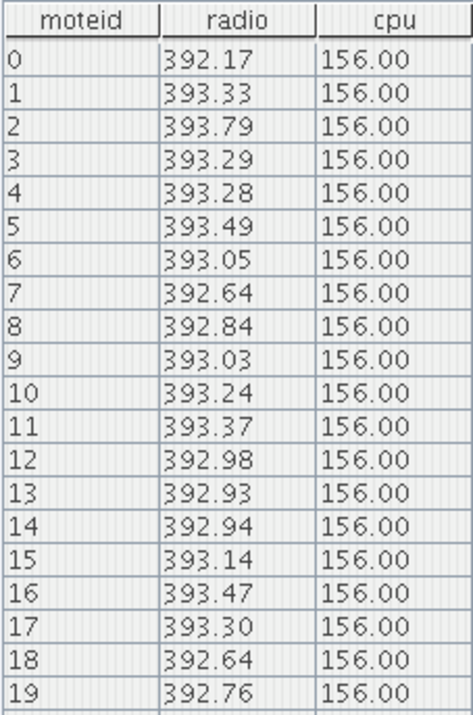
\includegraphics[width=3cm, height=5cm]{power_usage_avg_op}&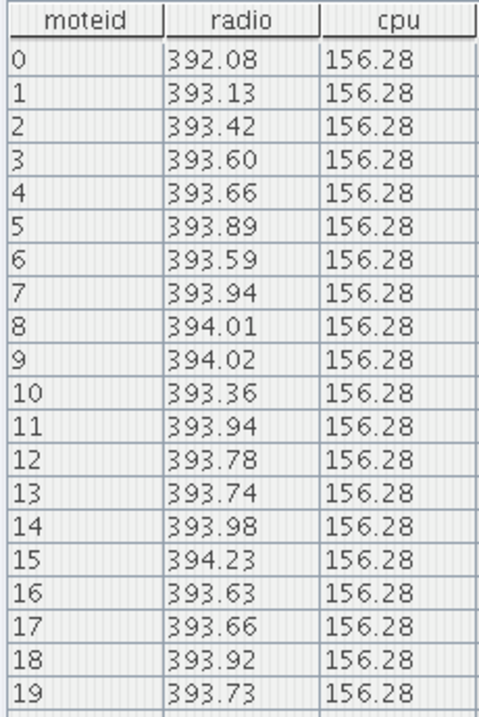
\includegraphics[width=3cm,
  height=5cm]{power_usage_with_sha1}\\
    (A) & (B) \\
  \end{tabular}
\caption{Power profile for AVG (A) and SecureSum (B)} 
\label{fig:avg}
\end{figure}

\subsubsection{Difficulties of SIA's result-checking phase in TinyDB}

In TinyDB and in real life WSN applications, data cannot be always fully aggregated
from all motes in the network. For instance, the count returned in SecureSum function 
in all of our experiments hardly reach 20, which is the number of motes. Meanwhile,
the result-checking phase of \cite{Chan06} is to ensure that all motes contribute
to the final result. A compromised aggregated mote can just say it has not received
messages from certain motes, or those messages comes late after the timeout to
send results back to the root. 

Another problem is that in TinyDB, the aggregation tree topology is changed 
frequently and it is hard to keep track of previous state of the tree to issue
off-path values for result-checking.

\subsubsection{Comments}

In general, the assumptions in SIA as well as other protocols for secure data aggregation
in WSN at the moment are too ideal and cannot deal with rapid changing and uncertainties
in WSN. In our opinion, it is more practical to look into cheap alternative for current
security primitives such as hashing, MAC, en/decryption, etc., to efficiently secure
the WSN given that attackers has limited power and time to make serious impact
on this real time environment. 

\section{Related Work}
\label{sec:relatedwork}

To provide ourselves with sufficient background in WSN research, we performed
a comprehensive survey of the field. We looked at many different protocols and
theories on WSN secure aggregation. This section will give an overview of what
we studied.

\subsection{Security Goals}

During WSN aggregation, there are several security goals we want to try to
meet. (see section 2.1 of survey paper)

\subsection{Types of Attacks}

Due to the nature of node deployment, the inexpensive cost of nodes, and many
other factors, WSNs are vulnerable to many types of attacks. We will briefly
overview each type of attack, and how it pertains to secure aggregation.\\

{\bf Denial of Service Attack (DoS)} \\
WSNs face the same vulnerability to DoS attacks that other wireless
networks face. An adversary can broadcast radio signals that interfere with
the frequencies used by the nodes, jamming the communications. In the context
of aggregation, if a node cannot communicate with its parents it will not be
able to pass on aggregated data.

{\bf Node Compromise} \\
Due to the low cost of each node, not much physical security is built into
them. This, along with the tendacy to deploy nodes in hostile territories,
leads to a high risk for node compromise. An adversary can capture a node,
dissect it and gain information such as its keys. In secure aggregation,
knowing an adversary can have access to any node and its keys makes ensuring
correct results considerably more difficult.

{\bf Sybil Attack} \\
A sybil attack is when an attacker can present itself as multiple identities
in the network. This can affect aggregation in multiple ways. The most
straightforward way would be to report multiple readings. Other methods
include fooling witness schemes into thinking enough witnesses have vouched
for a particular node, and generating enough votes to falsely elect a
compromised aggregator.

{\bf Selective Forwarding Attack} \\
Related to node compromise, a node under the control of an attacker can choose
which packets it wants to forward, and which it wants to simply ignore. In
certain aggregation schemes, such an attacker could forward enough packets to
look active, but still affect the aggregation results.

{\bf Replay Attack} \\
Without even having control of a node, an attacker can record traffic from the
network and rebroadcast it later, without necessarily understanding its
contents. This attack, although not particularily sophisticated, can cause
confusion and affect the manner in which aggregation results are collected.

{\bf Stealthy Attack} \\
The most dangerous type of attack, in a stealthy attack the attacker's goal is
not to simply disrupt the network, but to cause the base station to accept
false aggregation results. This can be accomplished by using one or more of
the above methods of attack, and results in the base station trusting and
accepting aggregation results that are not valid.

\subsection{SDA - Secure Data Aggregation}

Hu \& Evans propose the first secure data aggregation protocol in
\cite{SDA}. The security goals of SDA are to prevent intruders from being able
to inject forged readings, and prevent a single compromised node from being
able to report false aggregation results. These goals are achieved by using
delayed aggregation and authentication. Rather than having each parent
aggregate their children's results, the data and a MAC of the data are
forwarded up one more level and then aggregated. This way the grandparent can
check to make sure that the data hasn't been changed. During the verification
stage, the base station uses $\mu$Tesla to broadcast the temporary keys used
by each node so that their neighbors can authenticate messages previously
transmitted.

One negative of this protocol is that if two successive nodes (i.e. parent and
child) are corrupted then the protocol is broken. Also, once a grandfather
node detects node corruption it cannot tell which node, the child or the
grandchild, is corrupted. It also requires a fair amount of transmission, to
broadcast the temporary keys each round.

\subsection{ESA - Efficient secure aggregation in sensor networks}
Jadia \& Mathuria improve upon SDA in \cite{ESA}. Rather than use $\mu$Tesla
to have the base station broadcast the temporary keys used by each node, ESA
uses pairwise keys to encrypt data between nodes. Parent and child use one-hop
pairwise keys and grandparent and grandchild use two-hop pairwise keys. This
reduces communication from the base station and reduces storage because each
node doesn't need to hold onto data until they receive the temporary
keys. However, the protocol still breaks down if two successive nodes are
compromised.

\subsection{WDA - A witness-based approach for data fusion assurace in wireless sensor networks}

\subsection{SecureDAV - A secure data aggregation and verification protocol for sensor networks}

\subsection{SRDA - Secure reference-based data aggregation protocol for wireless sensor networks}

\subsection{CDA - Concealed data aggregation for reverse multicast traffic in sensor networks}

\subsection{EDA - Efficient Aggregation of Encrypted Data in Wireless Sensor Networks}

\subsection{SIA - Secure information aggregation in sensor networks}

Przydatek et al. in \cite{SIA} proposed a new framework for secure information
aggregation in sensor networks, named SIA. This framework uses a single
aggregator to locally collect and aggregate data. It then sends it to a home
server, which can prove with high probability that an accepted result is close
to the actual measurement. In SIA, the home server and aggregator each have a
master key, which they use to derive shared keys with each of the sensor
nodes. This allows for authenticated communication and, if necessary,
encryption. The home server and base station are assumed to have the ability
to broadcast authentic messages (such as queries) into the network. This can
be achieved using the $\mu$TESLA broadcast authentication protocol.

The security goal of SIA is to prevent {\em stealthy attacks}, where attackers
want to make the user accept false results, significantly different from the
actual measured results, without the user knowing. This is accomplished
through their proposed approach of {\em aggregate-commit-prove}. This is a
three phase process which allows local aggregation (saving expensive network
transmissions) and allows the home server to detect if the aggregator or a
sensor node is cheating.

The aggregator first collects data from sensors and computes the aggregation
result. Secondly, it commits to the data by constructing a Merkle hash tree
from the data. In such a tree, each node is computed as the hash of the
concatenation of its two child nodes. The root node is the {\em commitment} of
the collected data because, once it is computed, the values of the data cannot
be changed. Finally, the aggregator and home server engage in an interactive
proof phase. In this phase, the home server checks if the committed data is an
accurate respresentation of the actual sensor data, exposing any cheating
aggregators. This allows the home server to know with high probability whether
it should accept the aggregated results.

\subsection{SDAP - A secure hop-by-hop data aggregation protocol for sensor networks}

In \cite{SDAP}, Yang et al. outline a secure data aggregation protocol called
SDAP using the ideas of divide-and-conquer and commit-and-attest. In SDAP, all
sensor nodes contribute readings to the aggregation and some also do
aggregating. This is in contrast to SIA, where only the leaf nodes collect
environmental data. Privacy is afforded by symmetric keys shared between
neighbors, which encrypt and decrypt data on a hop-by-hop basis. Commitments
are achieved through MACs, using a key shared with the base station. In this
way, SDAP is similar to SIA and its Merkle hash trees. All sensor nodes
contribute readings to the aggregation and some also do
aggregating. Divide-and-conquer helps cycle aggregators, which helps
distribute both trust and power consumption more uniformly throughout the
network.

In a WSN tree structure, nodes closer to the root require more trust since
they aggregate the readings of a larger number of sensor nodes. In reality,
all of the sensor nodes will be the same, regardless of their distance from
the root. With this in mind, SDAP uses a divide-and-conquer approach to
separate the WSN network into multiple {\em logical subgroups}, which has the
effect of spreading trust more uniformly throughout the WSN. The groups are
formed dynamically while aggregation is taking place. If the current node
meets a specific criterion relating to the total number of readings it is
aggregating, that node becomes a {\em leader} node. The leader node represents
the root of the logical subgroup. The data aggregated by the leader is marked
as finished and is forwarded by subsequent nodes without aggregating further
on its path to the base station.

After the base station receives the results from each of the logical
subgroups, it can detect suspicious groups using a probabilistic method
(Grubbs' Test) \cite{Grubb} that detects outliers. Once a suspicious group has
been identified, that group can be targeted for verification. In the
verification phase, the leader of the suspicious group recursively forms a
path down to one of its leaves. Each member of the path and {em off path
  nodes} forwards its data back to the base station, encrypting with a key
shared with the base station. The base station can then recalculate the
commitment and check its integrity.

The downsides of SDAP are its hop-by-hop encryption, large amounts of
data transmission, and unbalanced logical subgroups (subgroups
depend on number of nodes and become uniform in size, but this does
not have guarantees on the balance of their trees).



\section{Background}
\label{sec:background}
\subsection{TESLA and $\mu$TESLA}

TESLA is an authenticated streaming broadcast protocol. It uses asymmetric
encryption, not suitable for sensor networks that have very limited
power. Instead, $\mu$TESLA is often used for authenticated broadcasting in
WSN. $\mu$TESLA is the "micro" version of TESLA. It uses delayed key
disclosure and one-way function key chains. These techniques allows WSN
network to achive asymmetric mechanism through a delayed disclosure of
symmetric keys. Because receiver does not know the key when receiving the data
and MAC (the key is only known by the base server), it is asymmetric
mechanism. Keys used by MACs use normal symmetric encryption.


\subsection{TAG - A tiny aggregation service for ad-hoc sensor networks}

TAG describes basic concepts involved in the process of initiating aggregation
in sensor networks. It does not worry about security issues. It abstracts the
low level details of sensor networks and provides a high level interface in
the form of a SQL query language for extracting information from a sensor
network. This SQL style query language by TAG gives power and time efficient
distribution of queries. Queries in TAG use only one table called {\em
  sensors}.

TAG uses a routing tree. It is not concerned with the details of setting up
this tree or ad-hoc routing in general. The ad-hoc network must fulfill the
requirements that each node has a route to the root and each node should not
receive duplicate messages.

The algorithm provided by TAG has two phases. First is the query distribution
phase. Distribution means queries are pushed down to the network. Second is
the collection phase. In this phase, only a single aggregate value will be
produced per epoch, or time period, for which information is repeatedly
collected.

This is an example of a query in TAG:

\begin{verbatim}
	SELECT AVG(volume), room FROM sensors
	WHERE floor = 6
	GROUP BY room
	HAVING AVG(volume) > threshold
	EPOCH DURATION 30s
\end{verbatim}

EPOCH DURATION is reporting interval. If it is 30s, sensors report their
reading in every thirty seconds. It works with the current TinyOS event driven
model. Authors say that the EPOCH DURATION clause saves substantial power
because nodes can sleep while knowing that their children will not be
transmittingd data.

\subsection{TinyOS/TinySIM}
Developed by the University of California, Berkley, TinyOS is the most popular
wireless sensor network operating system \cite{TinyOS}. Over 5000 research
groups use TinyOS for their research in WSN. TinyOS also forms the largest
sensor network community.

Because TinyOS is open source, we can analyze all of the implementations of
network protocols, MAC protocols, sensor interface, and other security
protocols.  TinyOS supports secure protocols for sensor networks (SPINS) which
provide $\mu$TESLA. TinyOS also supports a link-layer security module named
TinySec \cite{Karlof04}.  Link-layer encryption takes place in the lowest
protocol layers (layers 1 and 2 in the OSI model). It is not feasible over the
internet but is currently used by a number of organizations such as the
military.

TinyOS has event driven and state change methods. Each TinyOS application has
several independent modules, and an application is formed by connecting these
modules together.

TinySIM is a simulator for TinyOS. We can inject network packets that we want
to simulate for a WSN using TinySIM. TinyViz is a visualization tool for
TinySIM.

\subsection{Secure hierarchical in-network aggregation in sensor networks}

Chan et al. in \cite{Chan06} proposed an extended version of the SIA paper
above which uses the {\em aggregate-commit-prove} framework in a hierarchical
network. After aggregation, the base station checks the results by sending
verification data down the tree to every node to verify that every node's data
is actually counted. Each node on the path and the {\em off-path vertices'}
data will be sent to the base station.  In order to save communication cost of
verification, while aggregating data, some data need to be {\em
  delayed-aggregated} so that the logical aggregation tree is balanced.  The
idea is that some aggregators may aggregate the data of only some of its
subtrees and forward data from other subtrees to it parent node. Forwarded
data will be aggregated at higher level node so that it is logically a child
of this higher level node. The resulting logical tree will be a more balanced
tree.

\section{Proposed protocol}
\label{sec:protocol}

\subsection{Motivation}

\cite{SIA} and \cite{Chan06} provide an efficient framework for secure data
aggregation in WSN for protecting against false data injection. If a
compromised node is higher in the aggregation tree, i.e., closer to the root,
it will have more impact on the final result and may deviate the result on a
large scale.  In that case, the results are usually rejected even if a large
amount of nodes in the WSN are uncorrupted nodes. \cite{SDAP} addressed this
problem under their SDAP framework using a divide-and-conquer approach by
forming subgroups in the WSN and passing on aggregated data of group leaders
to the base station. This, in some sense, is similar to the
delayed-aggreagation approach in \cite{Chan06} for efficient verification of
aggregated results. The difference is data from group leaders would not be
aggregated at higher levels while in \cite{Chan06} data is passed on until a
balanced tree can be formed.

The two methods are compatible to each other and can be combined to get the
best of them. Inspired by this, we will employ the divide-and-conquer approach
within the SIA framework to make it more robust to attacks, especially when
corrupted nodes are at high level in the aggregation tree. At each aggregation
step in SIA framework, both the probability function in \cite{Chan06} and the
criteria to form a balanced tree in \cite{SDAP} will be used together to form
logical subgroups in the forms of balanced trees. The next section will give a
detailed explanation of our proposed protocol.

\subsection{Protocol description}

The proposed protocol is based on \cite{Chan06} and methods mentioned
in section \ref{sec:background}. Most of the steps in the proposed protocol
were worked out, but some of them still need more analyzing and researching.

First, TAG \cite{tag} is used to construct the aggregation tree in the WSN
from sensor nodes to base station. After this step, all nodes will know which
node to send their data to for aggregating as well as verifying the
results. TAG is considered to be a standard method in all protocols that we
have studied. In this step, we also use it unmodified but we may also look
into customizing it to create a more balanced aggregation tree to reduce the
cost of achieving balance in the the aggregation step.

Second, for query dissemination, we use $\mu$TESLA \cite{SPINS} for
authenticated broadcasting from the base station to every node in the
network. Like TAG, $\mu$TESLA is also a widely used method for this task in
many secure protocols for WSN.

Third, in the aggregation step, in our protocol, which is based on SIA, every
node will commit their values to parent node using a Merkel hash tree
\cite{Merkel} as in \cite{SIA}. The new feature that we propose is employed in
this step.  Subgroups of balanced trees are dynamically created while
aggregating data based on {\it (i)} a probability function, which depends on
the count of sensing child nodes at the current node, and {\it (ii)} the depth
of its subtrees. The node will be a group leader, and its data will be passed
on to the base station without being aggregated if the output of the
probability function is larger than a threshold and a balanced tree can be
formed from its subtrees. In this step, we do not use a cryptographic function
to encrypt aggregated data. However, privacy can be protected by using a
homomorphism primitives such as \cite{Castel} or similar methods. We may
analyze the increase in communication as well as computation cost when using
encryption in this step if time permits.

In the last step, final results will be verified using either the
prove-procedures in \cite{SIA} or the outlier detection and attest approach in
\cite{SDAP}. We still need to do more research to consolidate our knowledge of
the methods with detailed procedures and their costs to come up with clear a
description of this step to do experiments and put it in our final report.

\section{Evaluation}
\label{sec:evaluation}

For evaluation, we will implement the protocol and simulate attacks in
TinySim. We will measure the the number of rejections under attacks with
different thresholds for approximation. We will also analyze the cost of
communication of either choices for the last step our our protocol described
above. In addition, we hope that we can give some theoretical estimates on how
the protocol improved in terms of reducing rejections when the network is
attacked at high level nodes.

\section{Summary and status}
\label{sec:summary}

We proposed a combination of SIA and SDAP for robust secure data aggregation
in WSN. Compared to our milestone in previous report, we are a little late as
we haven't decided on the last past of the protocol yet, but other parts have
been worked out especially the aggregation step where SIA and SDAP are
combined. WSN is new to all group members so more time is spent on getting the
background than it was planed.

Our work distribution is as followed:

Brian Kleinke: 7 Hours. Read and analyzed papers, group discussions, wrote
introduction interim report, edited interim report.

Matt Kokotovich: ~9 hours. Read, compare, and contrast papers, group meeting
and discussions, wrote SIA summary in interim report, edited tex formatting.

Matt Soukup: ~16 hours. Reading and analyzing papers, meeting and discussing
with group, writing SDAP summary, and proofreading this interim report.

Thanh Ngo: ~18 hours. Reading papers, discussing with group to find ideas,
writing proposed protocol section and editing this report.

Yulduck Sung: ~14 hours. Read papers, discussed with group to find ideas,
wrote summaries of TinyOs, TinySIM, TinySec, $\mu$TESLA and TAG.

\section{Appendix - Installation and compiling}
\label{sec:appendix}

Our source code is made available at \\
http://code.google.com/p/sectinydb/source/browse/.\\
To compile, a running
TinyOS system is required. The easiest way to obtain such system is downloading
the Xubutos VMWare image at\\
http://sing.stanford.edu/tinyos/dists/xubuntos-2.0-vm.tar.gz.
This is a Xubuntu system with TinyOS installed and configured for TinyOS-2.x.

TinyDB currently works with TinyOS-1.x, so everytime we open up a terminal
to run or compile TinyOS, we need to type \textbf{tos1} to re-configure it to 
TinyOS-1.1. The source code for TinyOS-1.1 is in /opt/tinyos-1.x. Our SVN
repository resembles the tinyos-1.x folder structure but with only folders that
has modified content due to the big size of the whole source code. One can check
out the repository and replace corresponding folders with ours. To compile and run,
one can follow the instruction given in section 9 in /opt/tinyos-1.x/doc/tinydb.pdf.
Our SecureSum function is available in the aggregator dropdown list. To view
the power profile, before running TinyDBApp, one needs to do "export DBG=usr1,power", 
run TinyDBApp with option "-p" and run TinyViz to view the profile
by typing "tinyviz" in a terminal. 


% References should be produced using the bibtex program from suitable
% BiBTeX files (here: strings, refs, manuals). The IEEEbib.bst bibliography
% style file from IEEE produces unsorted bibliography list.
% -------------------------------------------------------------------------
\bibliographystyle{IEEEbib}
\bibliography{report}

\end{document}
